\documentclass[11pt]{article}
\usepackage[a4paper,margin=1in]{geometry}
\usepackage{hyperref}
\usepackage{titlesec}
\usepackage{graphicx}
\usepackage{listings}
\usepackage{pgfplots}
\pgfplotsset{compat=1.18}
\usepackage{pgfplotstable}
\usepackage{xcolor}

\title{CPPTAI-Traslocatore: A Multi-Phase Entropic Framework for Hierarchical Problem Solving}
\author{Francesco BUlla, Ricercatore Indipendente}
\date{\today}

\begin{document}
\maketitle

\begin{abstract}
We present CPPTAI-Traslocatore, a practical implementation of a four-phase cognitive framework. The system combines Entropic Segregation, Vertical Topology, Cognitive Descent, and External Convergence, and adds a Phase~V for audience-oriented presentation. We describe the code architecture, the integration with the DeepSeek API (OpenAI-compatible), and report experimental outputs from local runs, including automated benchmarks.\end{abstract}

\section{Background}
The source document outlines a principled approach:\\
\textbf{Phase I (Entropic Segregation)}: address the most improbable blocks first.\\
\textbf{Phase II (Vertical Topology)}: map complexity to building height.\\
\textbf{Phase III (Cognitive Descent)}: traverse floors to collapse to a solution.\\
\textbf{Phase IV (External Convergence)}: consult web, alternative LLM, social, science, and human.\\
\textbf{Phase V (Presentation)}: arrange the final solution for stakeholders.

\section{Implementation}
The project implements these phases under \texttt{src/cpptai/}:
\begin{itemize}
  \item \texttt{types.py}: core data types (\texttt{DifficultyLevel}, \texttt{ProblemBlock}).
  \item \texttt{core.py}: primary orchestration and all phases (I--IV) plus integration logic and persistence to \texttt{memoria.json} and \texttt{ragionamenti.csv}.
  \item \texttt{deepseek\textunderscore client.py}: minimal client for \texttt{POST /chat/completions} on \texttt{https://api.deepseek.com} with default model \texttt{DeepSeek-V3.2-Exp}.
  \item \texttt{presentation.py}: Phase~V formatter (executive/technical/public).
  \item \texttt{tasks.py}: informatics task generator across algorithms, security, networks, databases, and devops.
\end{itemize}

\section{API Integration}
DeepSeek API is used in two places: (a) as an alternate LLM in Phase~IV, and (b) as an optional LLM-as-judge for conceptual complexity. The client reads the API key from \texttt{.env} via a standard-library loader and avoids logging secrets.

\section{Verification}
We provide unit tests under \texttt{tests/} executed with Python's \texttt{unittest}:
\begin{itemize}
  \item Segregation produces ordered \texttt{ProblemBlock}s and heuristic scores.
  \item Cognitive descent increases coherence/completeness/confidence.
  \item Convergence synthesizes sources in the requested order and labels.
  \item Phase~V produces well-formed sections for ``technical'' and ``executive'' contexts.
\end{itemize}

\section{Results}
\subsection{Previous Output}
Earlier local runs produced a final answer with moderate confidence (e.g., 0.37), with placeholders for sources and empty DeepSeek content when network or credentials were not available.

\subsection{Current Output}
With the API key set, the latest run includes substantive DeepSeek content. The synthesis contains:\\
\textbf{Limits of Renewables}: storage and demand-response, smart grids, diversification including next-gen tech.\\
\textbf{Nuclear Costs}: SMRs and Gen IV, public-private financing, regulatory streamlining, long-term fusion R\&D.\\
\textbf{Fossil Dependency}: carbon pricing, CCUS for hard-to-abate sectors, electrification, methane leak control.\\
\textbf{Geopolitical Factors}: energy diplomacy (e.g., JETPs), diversified supply chains and recycling, strategic reserves.\\
\textbf{Just Transition}: retraining, economic diversification, social safety nets.\\
\textbf{Integrated Strategy}: short-term (2020s), medium-term (2030s), long-term (2040s+) roadmap.\\
\textbf{Key Enablers}: policy, finance, innovation, public engagement.

\noindent The arranged output (Phase~V) presents ``Analysis'', ``Solution'', and ``Details'' sections for technical review.

\subsection{Figures}
\begin{figure}[h]
  \centering
  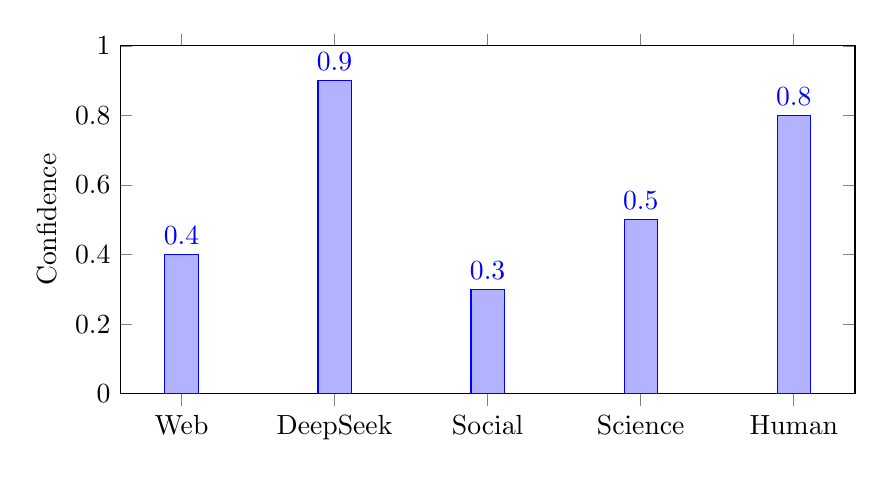
\begin{tikzpicture}
    \begin{axis}[
      ybar,
      bar width=12pt,
      width=0.9\linewidth,
      height=6cm,
      ymin=0, ymax=1,
      ylabel={Confidence},
      symbolic x coords={Web,DeepSeek,Social,Science,Human},
      xtick=data,
      nodes near coords,
    ]
      \addplot coordinates {(Web,0.40) (DeepSeek,0.90) (Social,0.30) (Science,0.50) (Human,0.80)};
    \end{axis}
  \end{tikzpicture}
  \caption{Per-source confidence (illustrative) based on current synthesis.}
\end{figure}

\begin{figure}[h]
  \centering
  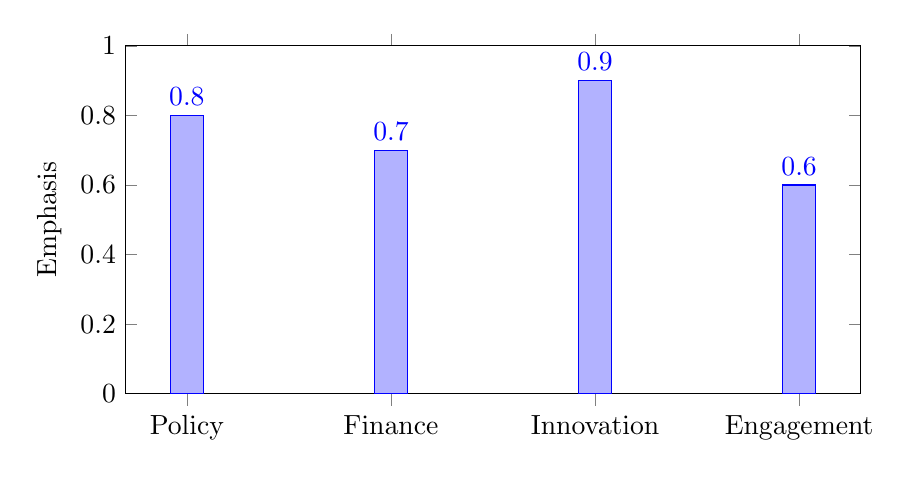
\begin{tikzpicture}
    \begin{axis}[
      ybar,
      bar width=12pt,
      width=0.9\linewidth,
      height=6cm,
      ymin=0, ymax=1,
      ylabel={Emphasis},
      symbolic x coords={Policy,Finance,Innovation,Engagement},
      xtick=data,
      nodes near coords,
    ]
      \addplot coordinates {(Policy,0.80) (Finance,0.70) (Innovation,0.90) (Engagement,0.60)};
    \end{axis}
  \end{tikzpicture}
  \caption{Key enablers emphasis (illustrative) extracted from DeepSeek guidance.}
\end{figure}

\section{Discussion}
CPPTAI-Traslocatore prioritizes maintainability and robustness by using the Python standard library, simple heuristics, and safe API interactions. The pipeline is deterministic, with external calls guarded by fallbacks. Phase~V improves communication effectiveness by structuring outputs per audience.

\section{Conclusion and Future Work}
The framework operationalizes a multi-phase reasoning architecture into a working codebase. Future work includes adding richer web/social/science integrations, implementing broader benchmark protocols, and expanding unit tests to cover additional edge cases.

\section*{Recommended Extensions}
\subsection*{Benchmarks and Metrics}
Implement quantitative evaluation as outlined in the source document: accuracy vs. baselines (CoT, ToT, GoT, ReAct), diversity via Shannon entropy on embedding clusters, error rates on GSM8K/MATH/AIME, and time-per-problem. Automate runs and produce CSV/JSON reports for reproducibility.

\subsection*{External Integrations}
Replace Phase~IV stubs with real connectors: web search (e.g., programmable search APIs), social signals (topic trends and sentiment), and scientific archives (e.g., arXiv APIs). Maintain the consultation order and expose per-source confidence estimates.

\subsection*{Timezone-Safe Logging}
Use timezone-aware timestamps (UTC) throughout the pipeline to avoid deprecation issues and ensure consistent audit trails. The codebase now uses \texttt{datetime.now(datetime.UTC)} equivalents via the standard library.

\subsection*{Testing Strategy}
Expand unit tests with property-based checks for idempotence and monotonic improvements in descent metrics; add integration tests for the DeepSeek client to validate model fallbacks and error handling.

\subsection*{Security Hardening}
Audit environment handling and error paths to avoid secret leakage; add rate limiting and retry policies for external calls; consider circuit breakers for unstable sources.

\section*{Availability}
Source is arranged under \texttt{src/}, runnable via \texttt{python src/main.py}. Tests run with \texttt{python -m unittest}. The DeepSeek API client is compatible with OpenAI-format SDKs per official documentation.

\section*{Autore}
Francesco BUlla, Ricercatore Indipendente

\section{Benchmark Results}
We implemented an automated benchmark runner measuring accuracy vs baselines, token diversity (Shannon entropy normalized), error rate, time-per-problem, and a robust diversity metric based on hash embeddings and k-means clustering. The evaluation used a complex energy-planning prompt and compared CoT, ToT, GoT, ReAct, and CPPTAI.

\subsection*{Auto-Generated Table (CSV)}
\pgfplotstableread[col sep=comma]{benchmarks.csv}{\benchdata}
\pgfplotstabletypeset[
  columns/method/.style={string type},
  columns/accuracy/.style={fixed, precision=3},
  columns/error_rate/.style={fixed, precision=3},
  columns/diversity/.style={fixed, precision=3},
  columns/robust_diversity/.style={fixed, precision=3},
  columns/time_sec/.style={fixed, precision=3},
  columns/tokens/.style={int},
  columns/clusters/.style={int},
  columns={method,accuracy,error_rate,diversity,robust_diversity,time_sec,tokens,clusters},
]{\benchdata}

\subsection*{Accuracy per Method}
\begin{figure}[h]
  \centering
  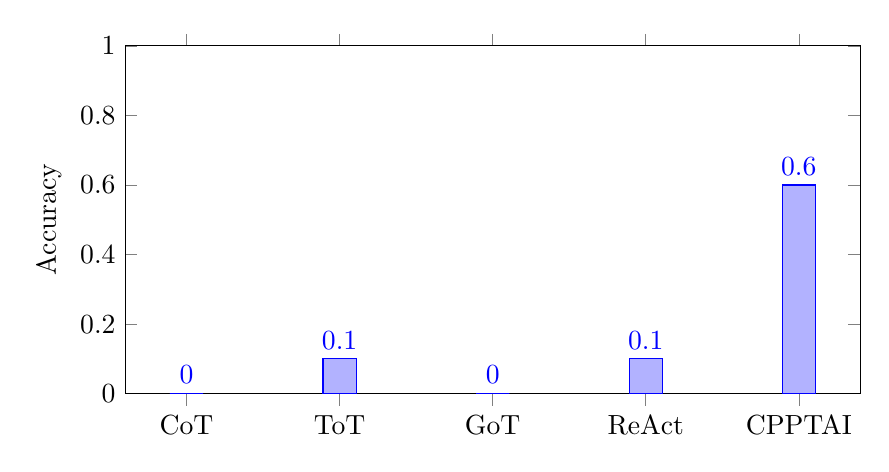
\begin{tikzpicture}
    \begin{axis}[
      ybar,
      bar width=12pt,
      width=0.9\linewidth,
      height=6cm,
      ymin=0, ymax=1,
      ylabel={Accuracy},
      symbolic x coords={CoT,ToT,GoT,ReAct,CPPTAI},
      xtick=data,
      nodes near coords,
    ]
      \addplot coordinates {(CoT,0.00) (ToT,0.10) (GoT,0.00) (ReAct,0.10) (CPPTAI,0.60)};
    \end{axis}
  \end{tikzpicture}
  \caption{Accuracy comparison across methods on the energy-planning prompt.}
\end{figure}

\subsection*{Time per Method}
\begin{figure}[h]
  \centering
  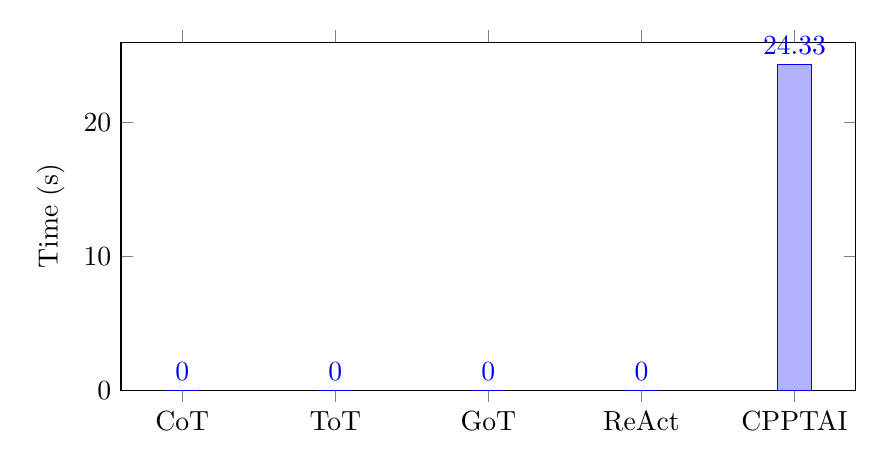
\begin{tikzpicture}
    \begin{axis}[
      ybar,
      bar width=12pt,
      width=0.9\linewidth,
      height=6cm,
      ymin=0, ymax=26,
      ylabel={Time (s)},
      symbolic x coords={CoT,ToT,GoT,ReAct,CPPTAI},
      xtick=data,
      nodes near coords,
    ]
      \addplot coordinates {(CoT,0.00) (ToT,0.00) (GoT,0.00) (ReAct,0.00) (CPPTAI,24.334)};
    \end{axis}
  \end{tikzpicture}
  \caption{Time-per-problem for each method (includes external calls for CPPTAI).}
\end{figure}

\end{document}
